\documentclass[10pt, a4paper, titlepage]{article}
\usepackage[margin=1in]{geometry}
\usepackage{graphicx, latexsym}
\usepackage{titling}
\setlength{\droptitle}{-25em}
\renewcommand{\maketitlehooka}{\Large}
\usepackage{setspace}
\usepackage{amssymb, amsmath, amsthm}
\usepackage[export]{adjustbox}
\usepackage{bm}
\usepackage{wrapfig}
\usepackage{epstopdf}
\usepackage{microtype}
\usepackage[hidelinks]{hyperref}
\usepackage{titling}
\usepackage{multirow}
\usepackage[table,xcdraw]{xcolor}
\usepackage{colortbl}
\usepackage{lscape}
\usepackage{float}
\usepackage[sort&compress,square,comma,authoryear]{natbib}
\hypersetup{
    pdftitle={Research Report Heleen Brüggen},
    pdfauthor={Heleen Brüggen},
    pdfsubject={Research Report Heleen Brüggen},
    pdfkeywords={},
    bookmarksnumbered=true,
    bookmarksopen=true,
    bookmarksopenlevel=1,
    colorlinks=false,
    pdfstartview=Fit,
    pdfpagemode=UseNone
}

\singlespacing

\begin{document}
\begin{titlingpage}
\begin{center}
\Huge\textbf{Master Research Report:  \\ Multilevel Multivariate Imputation by Chained Equations through Bayesian Additive Regression Trees} \\
\Large\textit{Methodology and Statistics for the Behavioural, Biomedical and Social Sciences}

\vspace{.5cm}

\normalsize\textit{Heleen Brüggen}

\vspace{15cm}

\begin{minipage}{0.5\textwidth}
\begin{flushleft}

\textbf{Word count:} \\
\textbf{Candidate Journal:} \\
\textbf{FETC Case Number:} \\
\textbf{Supervisors:} \\
MSc. T. Volker \\
Dr. G. Vink \\
 MSc. H. Oberman
\end{flushleft}
\end{minipage}%
\begin{minipage}{0.5\textwidth}
\begin{flushright}

3270 \\
Computational Statistics \& Data Analysis \\
23-1778 \\
------------------------\\
Utrecht University \\
Utrecht University \\
Utrecht University
\end{flushright}
\end{minipage}

\end{center}
\end{titlingpage}

\newpage

\section{Introduction}

Incomplete data is a common challenge in many fields of research. A frequent approach for dealing with incomplete data is listwise deletion, also known as complete-case analysis, which is to remove all incomplete cases from the data. However, this could possibly lead to biased results if the data is not Missing Completely At Random (MCAR), meaning the cause of the missing data is unrelated to the data \citep{buurenFlexibleImputationMissing2018, kang2013, enders2017, austin2021, rubin1976}. Furthermore, other approaches to dealing with incomplete data include: pairwise deletion, mean imputation and regression imputation, which also yield biased results \citep{buurenFlexibleImputationMissing2018}. Pairwise deletion, also known as available-case analysis, is to remove all incomplete cases from the analysis when considering a specific pair of variables. Pairwise deletion leads to unbiased results when correlation between variables are low and the data is MCAR. Mean imputation is to replace missing values with the mean of the observed values. Mean imputation will bias almost all estimates except the mean when the data is not MCAR. Regression imputation is to replace missing values with the predicted values from a regression model and is unbiased when the data is Missing At Random (MAR), meaning that the missing data is related to the observed data \citep{rubin1976}, and the factor influencing the missingness is present in the data \citep{buurenFlexibleImputationMissing2018}. So, in order to use these ad hoc strategies to deal with incomplete data correctly, the missing data mechanism should be carefully determined. However, determining the missing data mechanism is often difficult and MCAR is in practice an unrealistic assumption \citep{buurenFlexibleImputationMissing2018}. We can imagine that when a system becomes more complex, thus increases the amount of parameters, testing these assumptions also increases in complexity.

One of these complex systems are multilevel data structures. Multilevel data is hierarchically structured, where, for example, students are nested within schools, or patients are nested within hospitals \citep{hox2017, hox2011}. Thus, in these types of data sets there are level-1 and level-2 variables. Level-1 variables relate to the individual within a class and level-2 variables relate to the class as a whole. The recommended statistical technique to analyzing these models are multilevel models as it accounts for the specific dependencies in the  multilevel data sets \citep{hox2017, hox2011, ludtke2017}. It can contain both level-1 and level-2 variables, random intercepts, random slopes, and cross-level interactions \citep{hox2017, hox2011}.

Multiple imputation (MI) is considered a valid method for dealing with incomplete data and allows us the separate the missing data problem from the analysis problem \citep{mistlerComparisonJointModel2017, buurenFlexibleImputationMissing2018, enders2017, burgette2010, austin2021, audigier2018, vanbuuren2007, grund2021, hughes2014}. MI imputes each missing value in the data set more than once given the observed data, thereby considering necessary variation associated with the missingness problem. The multiply imputed data sets are analyzed, and the corresponding inferences are pooled according to Rubin's rules \citep{buurenFlexibleImputationMissing2018, austin2021, rubin1987, carpenter2013}.
Generally, multiple imputation operates under two frameworks: joint modeling (JM) and fully conditional specification (FCS) \citep{mistlerComparisonJointModel2017, buurenFlexibleImputationMissing2018, enders2018, enders2018a, hughes2014}. JM employs a multivariate data distribution and regresses incomplete variables on all complete variables to impute missing values. FCS, or chained equations, iteratively imputes one variable with missing values at a time through conditional univariate distributions regressing an incomplete variable on complete variables and previously imputed variables \citep{mistlerComparisonJointModel2017, buurenFlexibleImputationMissing2018, enders2016, enders2018, enders2018a, hughes2014, grund2018a}.

JM and FCS use multivariate and univariate linear mixed models respectively in a multilevel context \citep{mistlerComparisonJointModel2017, enders2018}. The implementation of JM and FCS in a multilevel context are equivalent in a two-level random intercept context with normally distributed data but differ beyond that \citep{enders2016, enders2018a}. Overall, FCS is believed to be more flexible than JM \citep{audigier2018, burgette2010, vanbuuren2007, grund2018a} and, thus, may be better suited for multilevel data. In FCS, one needs to define conditional models for all variables with missing values \citep{mistlerComparisonJointModel2017, buurenFlexibleImputationMissing2018, enders2018, enders2018a, enders2016, hughes2014, grund2018a} and the imputation models should at least be as general as the analysis model and preferably all-encompassing \citep{grund2018}. However, the complexity of the multilevel analysis model is built step-wise with non-linearities \citep{hox2017, hox2011}. Thus, defining imputation models for a multilevel data set is quite challenging \citep{buurenFlexibleImputationMissing2018, burgette2010, hox2011}.

% There are three ad-hoc strategies for dealing with multilevel missing data \citep{buurenFlexibleImputationMissing2018}. The first is listwise deletion, which will also lead to bias results if the data is not MCAR in a multilevel context \cite{grund2016, buurenFlexibleImputationMissing2018, ludtke2017}. Second is ignoring the multilevel structure and imputing the data as if it were a single-level data set. However, this will underestimate the Intra-Class Correlation (ICC) \citep{buurenFlexibleImputationMissing2018, ludtke2017, taljaard2008, hox2011}. The ICC can be interpreted as the expected correlation between two randomly sampled individuals from the same group or the proportion of the total variance at level-2 \citep{gulliford2005, shieh2012, hox2011}. The third strategy is fixed effect imputation: adding group dummy variables representing the group effects \citep{ludtke2017, enders2016}. Again, estimates in this method can be biased: the ICC will be overestimated and the between cluster regression coefficients will be underestimated \citep{ludtke2017, buurenFlexibleImputationMissing2018}.

Using non-parametric tree-based models as imputation models might solve this problem. Tree-based models use recursive partitioning to split the data into smaller subgroups based on the predictor variables maximizing the homogeneity of the subgroups. Tree-based models are non-parametric, which means that they do not assume a specific distribution of the data. Thus, they can handle non-linear relationships and interactions between the predictor variables well. Furthermore they handle continuous and catergorical variables simultaneously \citep{hill2020, burgette2010, lin2019, chipman2010, james2021, salditt2023, breiman1984}.

In a single-level imputation context, the use of tree-based, non-parametric models like regression trees, random forests or Bayesian Additive Regression Trees (BART) simplified imputation models and performed better than parametric methods: the imputations showed better confidence interval coverage of the population parameters, lower variance and lower bias, especially in non-linear and interactive contexts \citep{burgette2010, xu2016, silva2022}. Others have also found lower normalized root mean squared error (NRMSE), which in essence encapsulates the bias of the imputations, when imputing with a random forest algorithm compared to MICE and KNN imputation \citep{stekhoven2012, waljee2013}. Furthermore, they also found that the algorithm reduced computational time and could handle multivariate data consisting of both continuous and categorical data simultaneously.

BART models have also been implemented in a multilevel prediction context. However, multilevel-BART models (M-BART) have predominantly been implemented with random intercepts and no random slopes and cross-level interactions \citep{chen2020, wagner2020, tan2016, wundervald2022}. \citet{wagner2020} have found that this random intercept M-BART model provided better predictions with a lower Mean Squared Error (MSE) compared to a parametric multilevel model, \citet{tan2016} found higher Area Under the Curve values, and \citet{chen2020} found better predictions and better coverage compared to parametric models and a single-level BART model. Other researchers modeled the random intercept as an extra split on each terminal node within the BART algorithm and found a lower MSE compared to a standard BART model and parametric multilevel models \citep{wundervald2022}. \citet{dorie2022} developed a multilevel BART model that included random intercepts and random slopes by combining BART with the Stan algorithm. However, the random intercept and slope are modeled by Stan, which is a parametric method. Their results showed that their algorithm `stan4bart` showed better coverage of the population value and lower Root Mean Squared Error (RMSE) compared to BART models with varying intercept, BART models ignoring the multilevel structure, Bayesian Causal Forests (BCF), and parametric multilevel models.

In spite of these promising findings: tree-based model performing well in single-level imputation context \citep{burgette2010, xu2016, silva2022, stekhoven2012, waljee2013} and M-BART models performing well in a multilevel prediction context \citep{chen2020, wagner2020, tan2016, wundervald2022, dorie2022}, M-BART models have yet to be implemented in a multilevel multiple imputation context. Thus, my research question will be: \textit{Can multivariate imputation by chained equations through a multilevel bayesian additive regression trees model improve the bias, variance and coverage of the estimates in a multilevel context compared to current practices?} Given the success of non-parametric models in single-level multiple imputation, I anticipate that employing multilevel BART models in a multilevel missing data context will reduce bias, accurately model variance, and improve estimate coverage compared to classical multilevel imputation through \textit{2l.pmm, 2l.lmer, 2l.pan, 2l.jomo, rf} and single-level \textit{pmm} and complete case analysis in the R-package MICE \citep{buuren2011}.

This research report is organised as follows: in section 2, will contain some theoretical background and describe the methods in which I will implement the M-BART model in a multilevel imputation context and Section 3 will provide some preliminary results.

\section{Method}

\subsection{Theoretical background}
Bayesian Additive Regression Trees (BART) is a sum-of-trees model proposed by Chipman et al. \citep{chipman2010}. Regression trees are its building blocks \citep{chipman2010, hill2020, james2021}. Regression trees model non-linearities well and automatically through recursive binary partitioning of the predictor space \citep{hill2020, burgette2010}. Recursive binary partitioning doesn't assume a specific data form; it divides the predictor space to maximize variance explanation by automatically identifying best fitting splits \citep{hastie2017, james2021, salditt2023}. BART models can be described as:

\begin{subequations}
\label{eq:BART}
\begin{align}
y_i &= f(\textbf{x}_i) + \epsilon_i, \tag{1.1} \\
y_i &= g(\textbf{x}_{i}, T_{1}, M_{1})+ g(\textbf{x}_{i}, T_{2}, M_{2}) + \dots + g(\textbf{x}_{i}, T_{k}, M_{k}) + \epsilon_i, \tag{1.2}
\end{align}
\end{subequations}

where $y_i$ is the outcome variable for person \textit{i}, $f(\textbf{x}_i)$ is the sum-of-trees many regression trees, and $\epsilon_i$ is the error term; $\epsilon \sim \mathcal{N}(0,\,\sigma^{2})$. $\textbf{x}$ are the predictors included in the model, $T_{k}$ is the k\textsuperscript{th} tree and $M_{k}$ is the collection of leaf parameters within the k\textsuperscript{th} tree \citep{chipman2010, hill2020, james2021}. Next to the sum-of-trees model, BART also includes a regularization prior that constrains the size and fit of each tree so that each contributes only a small part of the overall fit to prevent overfitting \citep{chipman2010, hill2020, james2021}. The Bayesian back-fitting Markov Chain Monte Carlo (MCMC) algorithm is used to obtain estimates from BART. It updates each tree, conditional on the remaining trees, their associated parameters and $\sigma$, by fitting a new tree to the partial residuals, $r_{i}$, perturbing the tree from the previous iteration. The partial residuals, $r_{i}$, are defined as:

\begin{subequations}
\label{eq:partialresiduals}
\begin{align}
r_i &= y_i - \sum_{k' < k} \hat{f}^{b}_{k'}(x_{i}) - \sum_{k' > k} \hat{f}^{b-1}_{k'}(x_{i}), \tag{2}
\end{align}
\end{subequations}

where $\hat{f}^{b}_{k'}(x_{i})$ is the prediction of the $k'$\textsuperscript{th} tree in the $b$\textsuperscript{th} iteration for person $i$. The M-BART model including a random intercept can be identified as:

\begin{subequations}
\label{eq:M-BART}
\begin{align}
y_{ij} &= \sum_{k=1}^{m} f(\textbf{X}_{ij}; T_{k}, M_{k}) + \alpha_{j} + \epsilon_{ij}, \tag{3}
\end{align}
\end{subequations}

where, now, $y_{ij}$ is the outcome variable for person $i$ in cluster $j$ and $\alpha_{j}$ is the random intercept for cluster $j$.

\subsection{Simulation study}
I will conduct a simulation study to examine the performance of the M-BART model in a multilevel multiple imputation context through FCS. I will compare the M-BART model to the following multilevel and single level imputation methods: \textit{2l.pmm, 2l.lmer, 2l.pan, 2l.jomo, rf} and \textit{pmm} in MICE \citep{buuren2011}.
The following five factors will be varied:
\begin{enumerate}
	\item \textit{Intraclass Correlation} (ICC = 0, .05, .3 and .5)
	\item \textit{Number of clusters} (J = 30 and 50)
	\item \textit{Within-cluster sample size}  ($n_{j}$ = 5, 15, 25 and 50)
	\item \textit{The Missing At Random (MAR) and Missing Completely At Random (MCAR) data rate} (0\%, 25\% and 50\%)
	\item \textit{Within-group effect size:} (size of the regression coefficients $\beta$ = .2, .5 and .8)
\end{enumerate}

\begin{table}[h]
\centering
\caption{Simulation design}
\label{tab:simulationparameters}
\begin{tabular}{l|l}
\textbf{Parameter}              & \textbf{Values} \\ \hline
Number of clusters              & 30, 50          \\
Within-cluster sample size      & 5, 15, 35, 50   \\
ICC                             & 0, .05, .3, .5  \\
Missing data mechanism          & MAR, MCAR       \\
Amount of missingness           & 0\%, 25\%, 50\% \\
Within-group effect size        & .2, .5, .8
\end{tabular}
\end{table}

All these values are realistic in practice and/or previously proposed \citep{gulliford1999, murray2003, hox2017, grund2018, enders2018a, enders2020}. The ICC can be interpreted as the expected correlation between two randomly sampled individuals from the same group or the proportion of the total variance at level-2 \citep{gulliford2005, shieh2012, hox2011}. For each combination of varying parameters, a 1000 replicated data sets will be generated.

The simulation study will be performed in R \citep{rcoreteam2023} with the package MICE \citep{buuren2011} to perform the FCS imputations, which I will enhance by integrating a multilevel BART model. FCS multilevel imputation methods \textit{2l.pmm, 2l.lmer, 2l.pan, 2l.jomo, rf} and \textit{pmm} in MICE and complete case analysis will serve as a benchmark. The population data-generating mechanism will be based on the following multilevel model:
\begin{subequations}
\label{eq:population}
\begin{align}
y_{ij} &= \beta_{0j} + \beta_{1j}X_{1ij} + \beta_{2j}X_{2ij} + \beta_{3j}X_{3ij} + \beta_{4j}X_{4ij} + \beta_{5j}X_{5ij} + \beta_{6j}X_{6ij} + \beta_{7j}X_{7ij} + \epsilon_{ij}, \tag{4} \\
\beta_{0j} &= \gamma_{00} + \gamma_{01}Z_{1j} + \upsilon_{0j}, \tag{4.1} \\
\beta_{1j} &= \gamma_{10} + \gamma_{11}Z_{1j} + \upsilon_{1j}, \tag{4.2} \\
\beta_{2j} &= \gamma_{20} + \gamma_{21}Z_{1j} + \upsilon_{2j}, \tag{4.3} \\
\beta_{3j} &= \gamma_{30} + \gamma_{32}Z_{2j} + \upsilon_{3j}, \tag{4.4} \\
\beta_{4j} &= \gamma_{40} + \upsilon_{4j}, \tag{4.5} \\
\beta_{5j} &= \gamma_{50} + \upsilon_{5j}, \tag{4.6} \\
\beta_{6j} &= \gamma_{60} + \upsilon_{6j}, \tag{4.7} \\
\beta_{7j} &= \gamma_{70}, \tag{4.8}
\end{align}
\end{subequations}
where $y_{ij}$ is a continuous level 1 outcome variable for person $i$ in group $j$ and $Z_{1j}$ and $Z_{2j}$ are continuous level 2 variables. The random intercept $\beta_{0j}$ is determined by the grand mean $\gamma_{00}$, the group effect $\gamma_{01}Z_{1j}$ and the group-level random residuals $\upsilon_{0j}$. The regression coefficients $\beta_{1j}$, $\beta_{2j}$, and $\beta_{3j}$ for the continuous variables $X_{1ij}$, $X_{2ij}$, and $X_{3ij}$ depend on the the intercepts $\gamma_{10}$, $\gamma_{20}$, and $\gamma_{30}$, the cross-level interactions $\gamma_{11}Z_{1j}$, $\gamma_{21}Z_{1j}$, and $\gamma_{32}Z_{2j}$, and the random slopes $\upsilon_{1j}$, $\upsilon_{2j}$, and $\upsilon_{3j}$. The regression coefficients $\beta_{4j}$, $\beta_{5j}$ and $\beta_{6j}$ are determined by the intercepts $\gamma_{40}$, $\gamma_{50}$ and $\gamma_{60}$ and the random slopes $\upsilon_{4j}$, $\upsilon_{5j}$ and $\upsilon_{6j}$. The regression coefficient $\beta_{7j}$ is determined by the intercept $\gamma_{70}$. The residuals and random slopes $\upsilon_{0j}$, $\upsilon_{1j}$, $\upsilon_{2j}$, $\upsilon_{3j}$, $\upsilon_{4j}$, $\upsilon_{5j}$, $\upsilon_{6j}$ and $\epsilon_{ij}$ follow a zero-mean normal distribution. The variance of $\upsilon_{0j}$, the group-level random residuals, were scaled such that the ICC value was as specified. $\upsilon_{1j}$, $\upsilon_{2j}$, $\upsilon_{3j}$, $\upsilon_{4j}$, $\upsilon_{5j}$, and $\upsilon_{6j}$ all have a variance of 1. $X_1$, $X_2$, $X_3$, $X_4$, $X_5$, $X_6$ and $X_7$ are multivariate normally distributed: $\mathbf{X}_{ij} \sim \mathcal{N}(\boldsymbol{\mu}, \boldsymbol{\Sigma})$, with $\boldsymbol{\mu} = (0, 0, 0, 0, 0, 0, 0)$ and $diag(\boldsymbol{\Sigma}) = (6.25, 9, 4, 11.56, 4, 2.5, 19.36)$ with no co-variances. The level-2 variables $Z_1$ and $Z_2$ are also multivariate normally distributed:  $\mathbf{Z}_{j} \sim \mathcal{N}(\boldsymbol{\mu}, \boldsymbol{\Sigma})$, with $\boldsymbol{\mu} = (0, 0)$ and $diag(\boldsymbol{\Sigma}) = (1, 2.56)$ with no co-variances.

The estimates will be evaluated on their relative bias (the difference between the average estimate and the true value), modeled variance and the 95\% confidence interval coverage \citep{oberman2023}, which will be calculated as follows \citep{morris2019}:
\begin{subequations}
\label{eq:evaluations}
\begin{align}
Bias &= \frac{1}{n_{\text{sim}}} \sum_{i=1}^{n_{\text{sim}}} (\hat{\theta}_i - \theta), \tag{5} \\
% MSE &= \frac{1}{n_{\text{sim}}} \sum_{i=1}^{n_{\text{sim}}} (\hat{\theta}_i - \theta)^{2}, \tag{6} \\
Coverage &= \frac{1}{n_{\text{sim}}} \sum_{i=1}^{n_{\text{sim}}} I({\theta} \in [\hat{\theta}_{\text{min},i}, \hat{\theta}_{\text{max},i}]), \tag{6} \\
SE &= \frac{1}{n_{\text{sim}}} \sum_{i=1}^{n_{\text{sim}}} \sqrt{\frac{\sigma^2_{\hat{\theta}_i}}{N}}, \tag{7}
\end{align}
\end{subequations}
where $\hat{\theta}_i$ is the estimated parameter, $\theta$ is the true value, $n_{\text{sim}}$ is the number of simulated data sets, $\hat{\theta}_{\text{min},i}$ and $\hat{\theta}_{\text{max},i}$ are the lower and upper bounds of the 95\% confidence interval, $\sigma^2_{\hat{\theta}_i}$ is the variance of the estimated parameter and $N$ is the size of each simulated data set.

In this research report, the preliminary results will pertain to the evaluation of different BART models in terms of the bias and MSE of the estimates. The MSE will be calculated as follows \citep{morris2019}:
\begin{subequations}
\label{eq:MSE}
\begin{align}
MSE &= \frac{1}{n_{\text{sim}}} \sum_{i=1}^{n_{\text{sim}}} (\hat{\theta}_i - \theta)^{2}, \tag{8}
\end{align}
\end{subequations}
where $\hat{\theta}_i$ is the estimated parameter, $\theta$ is the true value, and $n_{\text{sim}}$ is the number of simulated data sets. In order to reduce computational time, 6 data sets will be simulated for each scenario. Furthermore, since missing data mechanisms are not relevant for this research report, they will not be incorporated in the simulated data sets. 576 data sets will be simulated in total.
4 different models will be compared: a single level BART, single level BART with group-dummy's, a multilevel BART model incorporating a random intercept \citep{chen2020, wagner2020, tan2016, wundervald2022}, and a multilevel BART model combined with Stan to model the random parts of the models \citep{dorie2022}. The first three models will be performed in R \citep{rcoreteam2023} with the package \textit{dbarts} \citep{dorie2023} and the last will performed with the R-package \textit{stan4bart} \citep{dorie2023a}. The default arguments from the function \textit{rbart\_vi} will be used for all models, as well as the default priors.

\section{Results}
\graphicspath{{./graphs/}}

The results of this research report are shown in figure \ref{fig:biasplots} and \ref{fig:mseplots}. Figure \ref{fig:biasplots} shows the average relative bias for all models, simulated data sets, and every \textit{ICC} value. On the x-axis we can see the different simulated data sets with their names specifying the parameters used in generation. Figure \ref{fig:mseplots} shows the average Mean Squared Error (MSE) for all models, data sets and \textit{ICC} values.

In figure \ref{fig:biasplots} we can see that when there is no multilevel structure in the data set, $ICC = 0$, the models perform similarly in terms of relative bias: overall, the bias is around zero. We can see a slight increase in relative bias when the group size decreases, or more specifically, when the total sample size is small relative bias seems to slightly increase. When we increase the amount of multilevel structure in the data set, $ICC > 0$, we can see a divide in the performance of the models. Even with a little multilevel structure, $ICC = .05$, the single level BART model (bart) increases in relative bias. The single level BART model shows higher levels of relative bias when the total sample size is small. However, when the total sample size is large, 2500, the single level BART model performs better than the single level BART model incorporating a group-dummy. The same pattern is observed for the other models: when $ICC = .05$, the relative bias decreases when the total sample size increases. This pattern is further continued when increasing the \textit{ICC}: the relative bias decreases when the total sample size increases for both $ICC = .3$ and $ICC = .5$. However, when considering the stan4bart model, which models the random parts of the model in Stan and the fixed parts in BART, the relative bias stay considerably constant when increasing the \textit{ICC}. While the relative bias is higher when the total sample size is small, it does not seem to significantly increase when introducing more multilevel structure. This cannot be said for the bart and gbart models, which show a slight increase in relative bias when increasing the \textit{ICC}, especially in the lower total sample sizes. The rbart model, which incorporates a random intercept, shows a similar pattern as the stan4bart model, but with overall more relative bias.

\begin{figure}[H]
\caption{Bias of the estimates for all simulated data sets and multiple ICC values using four models. bart = single level BART model, gbart = single level BART model with group-dummys, rbart = multilevel BART model incorporating a random intercept, stan4bart = multilevel BART model combined with Stan to model the random parts of the models. Data set names show the number of groups, group size and within group effect size. Bias is based on 6 replicates for every data set.}
\centering
\label{fig:biasplots}
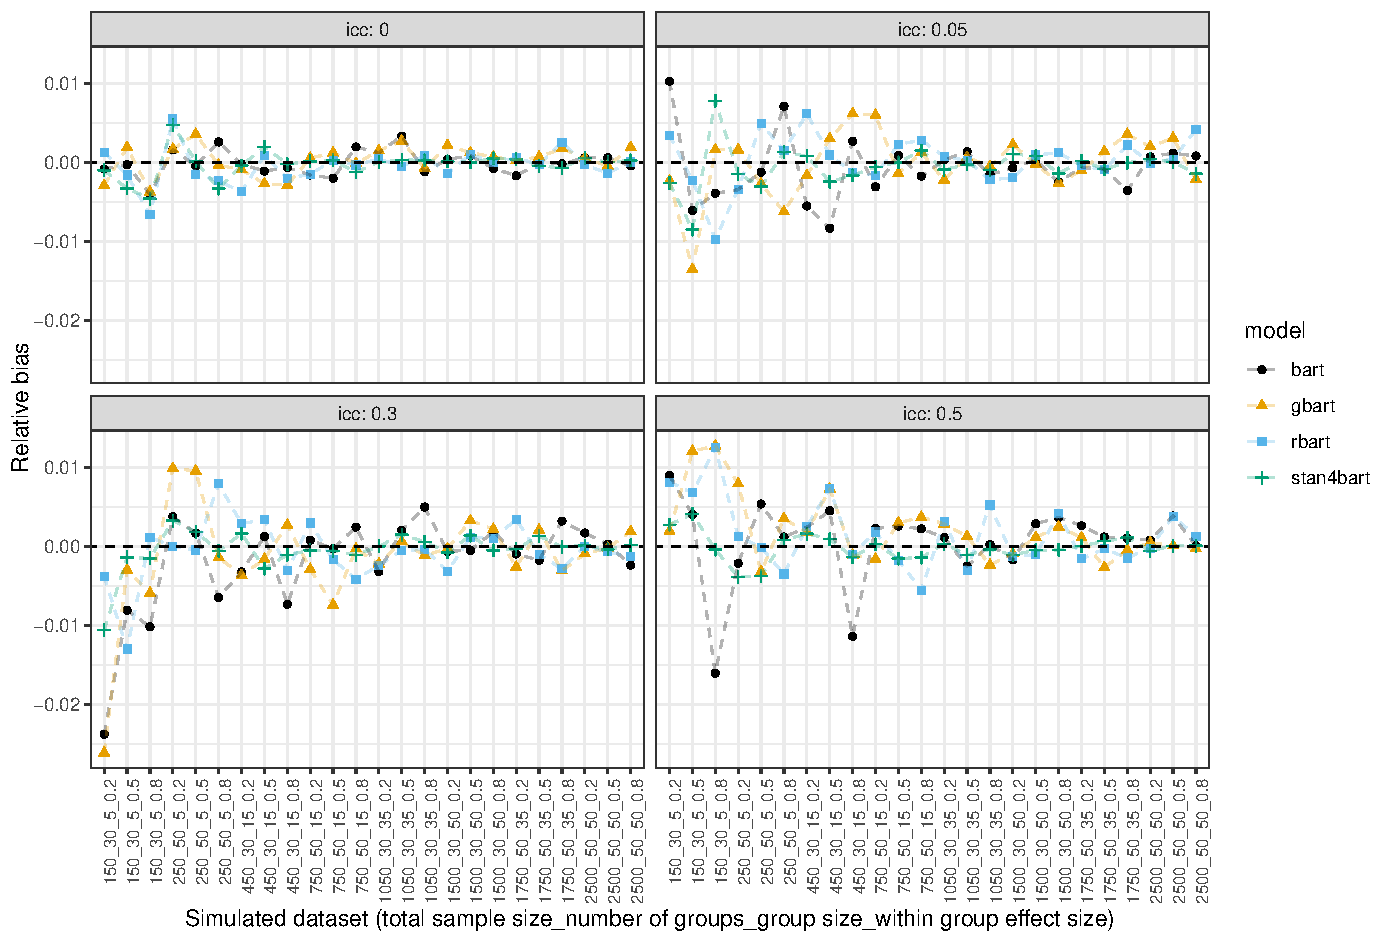
\includegraphics[width=\textwidth]{biasplots3.pdf}
\end{figure}

Figure \ref{fig:mseplots} shows a similar pattern as figure \ref{fig:biasplots}. When there is no multilevel structure in data sets, $ICC = 0$ the models perform well and almost exactly the same. When introducing multilevel structure, we can start to see a divide in the performance of the models. When $ICC = .05$ the models bart, gbart and rbart perform similarly, with gbart outperforming the other two models when the group sizes are 35 or larger. However, stan4bart consistently outperforms the other three models in terms of MSE. Introducing more multilevel structure to the data, $ICC = .3$, divides the performance of the models further: in small data sets bart now has the highest MSE with gbart performing only a little better. rbart performs better than bart and gbart, but when the data sets increase in size, it performs similar to bart with gbart outperforming them both. stan4bart is still the hast the overall lowest MSE. Increasing the \textit{ICC} further to .5 exaggerates these patterns. Over all \textit{ICC} values, increasing the within group effect size increases the MSE of the models.

\begin{figure}[H]
\caption{Mean Squared Error (MSE) of the estimates for all simulated data sets and multiple ICC values using four models. bart = single level BART model, gbart = single level BART model with group-dummys, rbart = multilevel BART model incorporating a random intercept, stan4bart = multilevel BART model combined with Stan to model the random parts of the models. Data set names show the number of groups, group size and within group effect size. MSE is based on 6 replicates for every data set.}
\centering
\label{fig:mseplots}
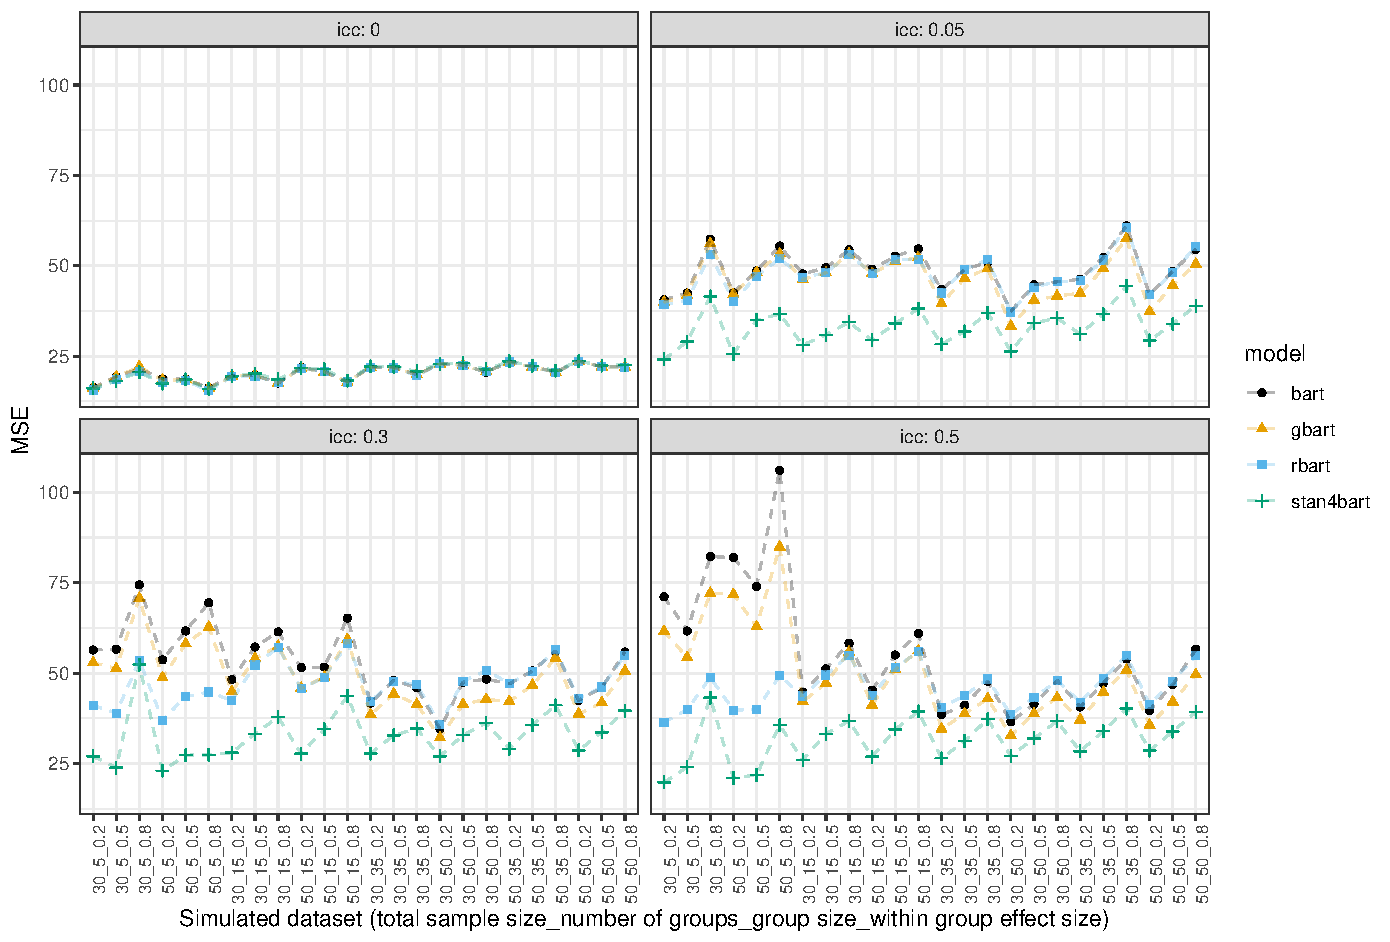
\includegraphics[width=\textwidth]{mseplots3.pdf}
\end{figure}

\newpage
\section{Discussion}

\newpage
\bibliography{thesis}
\bibliographystyle{apalike}

\end{document}

